\chapter{Introduction}
\label{cha:intro}

% Important: you have to switch to arabic numbering here!
\pagenumbering{arabic}

\textcolor{magenta}{
The following points should appear in the abstract and in more elaborate form in the introduction:
	\begin{enumerate}
		\item Machine Learning
		\item Text Analytics: detect word sense 
		\item Sense embeddings to represent word senses
		\item Polysemy: Multiple senses of a word. 
		\item What is the best way to do this? $\to$ multiple senses per word
		      $\to$ investigate and improve current methods with multiple senses per word
		\item Main Task of the thesis: Implementation of methods with multiple senses per word in Spark to be able to execute in parallel
		\item Train with Wikipedia corpus. Evaluate by inspecting similar word senses.  and evaluate similarity tasks.
		\item Improvement: better speed and better similarity
		\item organization of the thesis	
	\end{enumerate}	
}

\section{Distributed word representations}

\cite{git2010systematic}
%\cite{git2010systematic}
Machine learning approaches for natural language processing have to represent the words of a language in a way such that Machine Learning modules may process them. This is especially important for text mining, where data mining modules analyze text corpora. 

Traditional text mining analyses use the vector space representation \citep{SaltonWongEtAl1975}, where a word is represented by a sparse vector of the size of the vocabulary (usually more than 100.000), where all values are 0 except the entry for the actual word. This representation is also called \emph{One-hot representation}. This sparse representation, however, has no information on the semantic similarity of words.

Recently word representations have been developed which represent each word as a vector of $k$ (e.g. $k=100$) real numbers as proposed by \citep{CollobertWeston2008} and  \citep{MikolovSutskeverEtAl2013}. Generally, we call such a vector a \emph{word embedding}. By using a large corpus in an unsupervised algorithm word representations may be derived such that words with similar syntax and semantics have representations with a small Euclidean distance. Hence the distances between word embeddings corresponds to the semantic similarity of underlying words. These embeddings may be visualized to show comunalities and differences between words, sentences and documents. Subsequently these word representations may be employed for further text mining analyses like \emph{opinion mining} \citep{SocherPerelyginEtAl2013}, Kim 2014, Tang et al. 2014) or \emph{semantic role labeling} \citep{ZhouXu2015} which benefit from this type of representation \citep{CollobertWestonEtAl2011}.

These algorithms are based on the very important assumption that if the contexts of two words are similar, their representations should be similar as well \citep{Harris1954}.\com{please more details on this} Figure \ref{fig:neighbouring_words} shows how neighboring words determine the sense of the word "bank" in a number of example sentences. So many actual text mining methods make use of the context of words to generate embeddings. 
\begin{figure}[H]
\centering
\begin{minipage}{1.0\textwidth}
 
	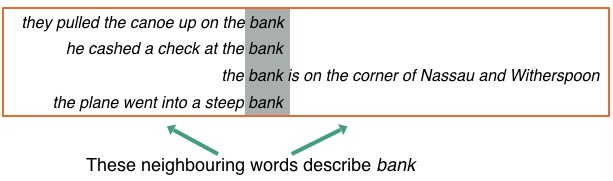
\includegraphics[width=1.0\textwidth]{neighbouring_words} 
	
\end{minipage}%
\label{fig:neighbouring_words}
\caption{Neigboring words defining the specific sense of "bank".}
\end{figure}	
A traditional approach to derive word embeddings is the analysis of the  word co-occurrence matrix \citep{DeerwesterDumaisEtAl1990}. It is based on the one-hot representation. Each row of the matrix represents the information of one word's context, which is sparse and huge. This matrix is decomposed using  singular value decomposition (SVD) to generate low-dimension embedding vectors. The context can be the occurrences of words in the corresponding document  or be the average occurrence's of surrounding words from all documents\com{I do not understand that}. 


Recently, artificial neural networks became very popular to generate lower-dimensional word embeddings. Prominent algorithms are \emph{Senna} \citep{CollobertWeston2008}, \emph{Word2vec} \citep{MikolovSutskeverEtAl2013} and Glove \citep{PenningtonSocherEtAl2014}. They all use randomly initialized vectors to represent words . Subsequently these embeddings are modified in such a way that the word embeddings of the neigboring words may be predicted with minimal error by a simple neural network function. 

\section{Polysemy}

Note that in the approaches described above each word is mapped to a single embedding vector. It is well known, however, that a word may have several different meanings, i.e. is \emph{polysemous}. For example the word "bank" among others may designate: 
\begin{itemize}
	\item the slope beside a body of water,
	\item a financial institution,
	\item a flight maneuver of an airplane.
\end{itemize}
Further examples of polysemy are the words "book", "milk" or "crane".
WordNet \citep{Fellbaum1998} and other lexical resources show, that most common words have 3 to 10 different meanings.
 Obviously each of these meanings should be represented by a separate embedding vector, otherwise the embedding will no longer represent the underlying sense. This in addition will harm the performance of subsequent text mining analyses. Therefore we need methods to learn  embeddings for senses rather than words.


\emph{Sense embeddings} are a refinement of word embeddings. For example, "bank" can appear either together with "money", "account", "check" or in the context of "river", "water", "canoe". And the embeddings of "money", "account", "check" will be quite different from the embeddings of "river", "water", "canoe". Consider the following two sentences 
\begin{itemize}
	\item They pulled the canoe up the bank.
	\item He cashed a check at the bank.
\end{itemize}
The word "bank" in the first sentence has a different sense than the word "bank" in the second sentence. Obviously, the context is different. 
So if we have a methods to determine the difference of the context, we can relabel the word "bank" to the word senses "bank$_1$" or "bank$_2$" denoting the slope near a river or the financial institution respectively. We call the number after the word the sense labels of the word "bank". This process can be performed iteratively for each word in the corpus by evaluating its context.

\com{An alternative representation of words is generated by topic models \citep{BleiNgEtAl2003}, which represent each word of a document as a finite mixture of topic vectors. The mixture weights of a word depend on the actual document. This implies that a word gets different representations depending on the context. Please elaborate}

In the last years a number of approaches to derive sense embeddings have been presented. \cite{HuangSocherEtAl2012} used the clustering of precomputed one-sense word embeddings and their neighborhood embeddings to define the different word senses. The resulting word senses are fixed to the corresponding word neighborhoods and their values are trained until convergence. A similar approach is described by \cite{ChenLiuEtAl2014}. Instead of a single embedding each word is represented by a number of different sense embeddings. During each iteration of the supervised training of Senna or Word2vec for each position of the word the best fitting embedding is selected according the fitness criterion\com{Please reformulate sentence}. Subsequently only this embedding is trained using back-propagation. Note that during training a word may be assigned to different senses thus reflecting the training process. A related approach was proposed by \cite{TianDaiEtAl2014}.

It turned out that the resulting embeddings get better with the size of the training corpus and an increase of the dimension of the embedding vectors. This usually requires a parallel environment for the execution of the training of the embeddings. Recently \emph{Apache Spark} \citep{ZahariaChowdhuryEtAl2010} has been presented, an opensource cluster computing framework. Spark provides the facility to utilize entire clusters with implicit data parallelism and fault-tolerance against resource problems, e.g. memory shortage. The currently available sense embedding approaches are not ready to use compute clusters, e.g. by Apache Spark. 

\section{Goal and Organization of the Thesis}

The main aim of this thesis is to derive expressive word representations for different senses in an efficient way. We will investigate sense assignment models which will extend known word embedding (one sense) approaches. Our goal is to implement such a method on a compute cluster using Apache Spark to be able to process larger training corpora and employ higher-dimensional sense embedding vectors.
\del{Our goal is not to introduce a very excellent method which can get the best sense embedding results, but to try the new model structure like sense assignment and the new software tool like distributed framework Spark to get the results reasonable and efficient.} 
Our main work will focus on the extension of Skip-gram model \citep{MikolovSutskeverEtAl2013} in connection to the approach of \citep{NeelakantanShankarEtAl2015} because these models are easy to use, very efficient and convenient to train. \del{And these days, some JVM based big data frameworks like Apache Spark are more and more popular, but the relative works on neural language processing especially word embedding and sense embedding use very few about these new techniques. That's the main reason that we try to use this new technique to implement our model.} When using the Spark big data framework, we want to gain some experience and get  feedback about the advantages and disadvantages of the new techniques.

\com{Rewrite this if the chapters are finished!}
In the next chapter, we will introduce relative word embedding methods and sense embedding methods. We start with the neural language model and explain the early models of word embeddings. And then we focus on the word2vec \cite{MikolovSutskeverEtAl2013} especially about Skip-gram model. There will be many mathematical details including gradient calculation. After that, we will introduce two famous sense embedding models based the above word embedding works. 
The chapter 3 is our model description for sense embeddings. We use the spark framework to implement our model. The chapter 4 will introduce our implementation and show the experiment we did including parameter comparison and word senses visualization. At last chapter conclusion, we will analysis the advantages and disadvantages about our methods including model and implementation and give some ideas about how we can improve it in the future and what else we can do.

